\subsection{Two Shower Sideband}
\label{sec:TwoShowerSideband}

This sideband is chosen to better understand the detector response to electromagnetic showers and the background induced by neutral pion production.

\todo[inline]{Find out why the "no uncontained showers" cut isn't used any more, and what the pi0 gammadot variable is.}

No pion background scaling is applied to the following plots.

\begin{figure}[H]
    \centering
    \begin{subfigure}{0.33\linewidth}
        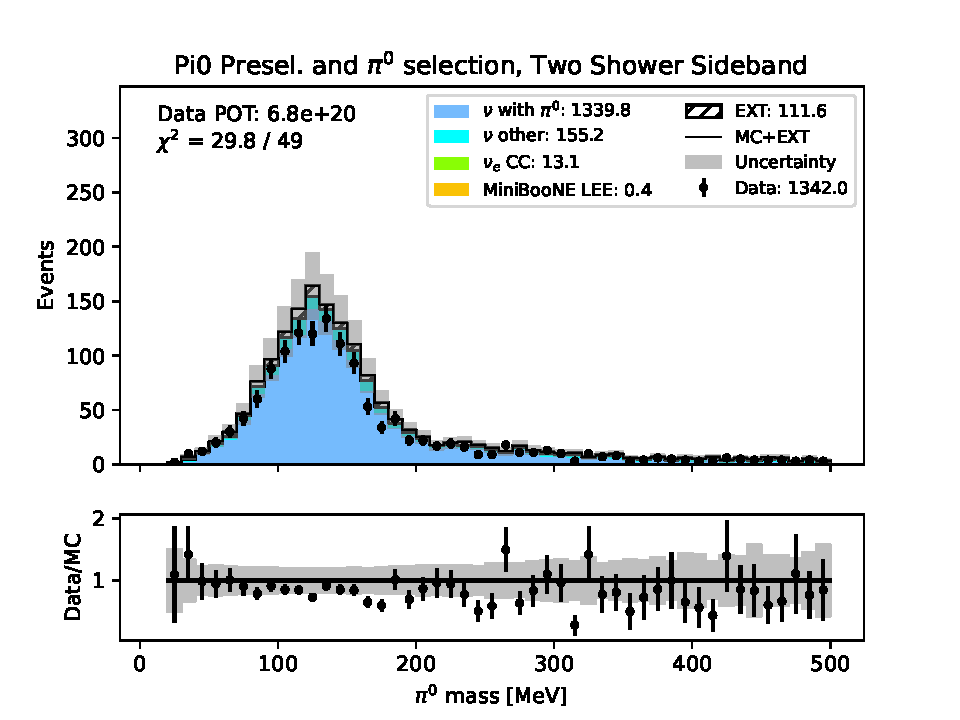
\includegraphics[width=\linewidth]{technote/Sidebands/Figures/TwoShowerSideband/two_shr_sideband_pi0_mass_Y_corr_run123_PI0_PI0.pdf}
        \caption{Reconstructed $\pi^0$ mass, runs 1-3.}
    \end{subfigure}%
    \begin{subfigure}{0.33\linewidth}
        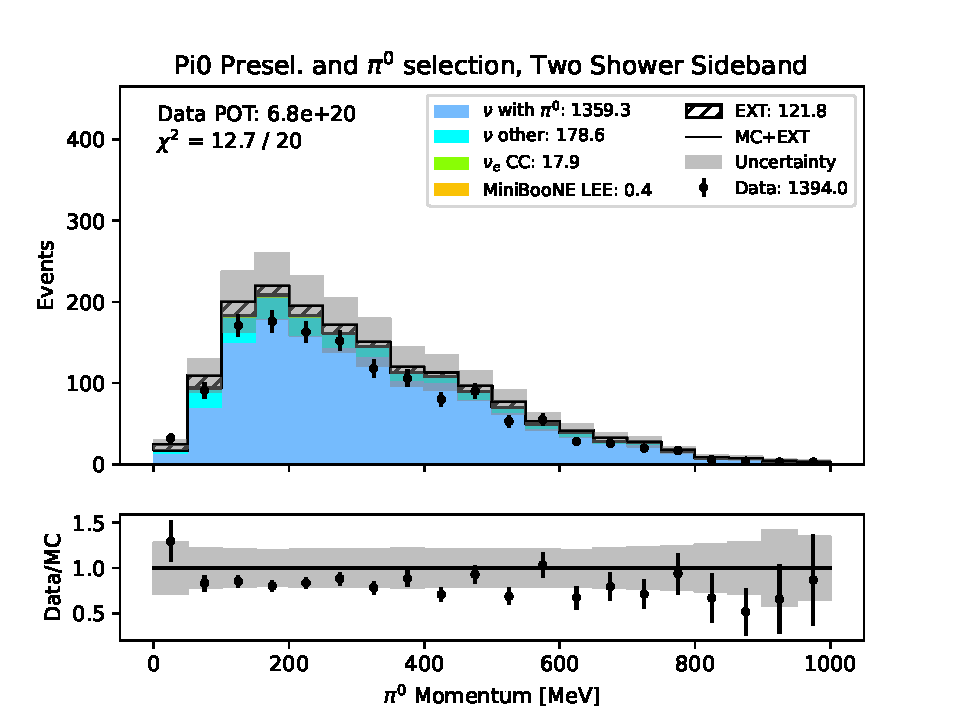
\includegraphics[width=\linewidth]{technote/Sidebands/Figures/TwoShowerSideband/two_shr_sideband_pi0momentum_run123_PI0_PI0.pdf}
        \caption{Reconstructed $\pi^0$ momentum, runs 1-3.}
    \end{subfigure}%
    \begin{subfigure}{0.33\linewidth}
        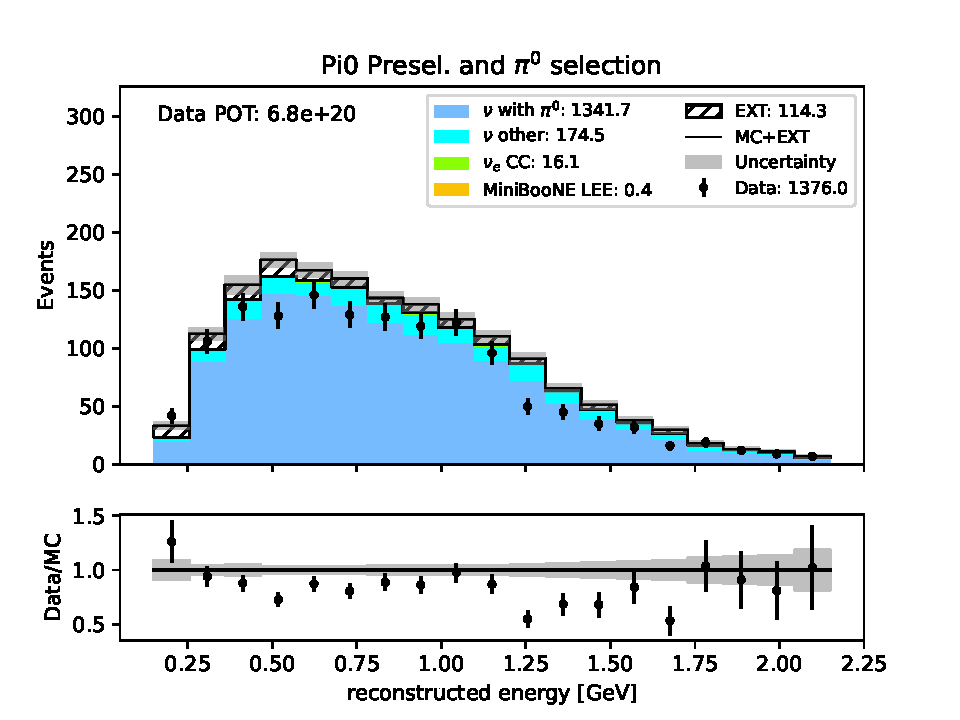
\includegraphics[width=\linewidth]{technote/Sidebands/Figures/TwoShowerSideband/two_shr_sideband_reco_e_run123_PI0_PI0.pdf}
        \caption{Reconstructed neutrino energy, runs 1-3.}
    \end{subfigure}
    \begin{subfigure}{0.33\linewidth}
        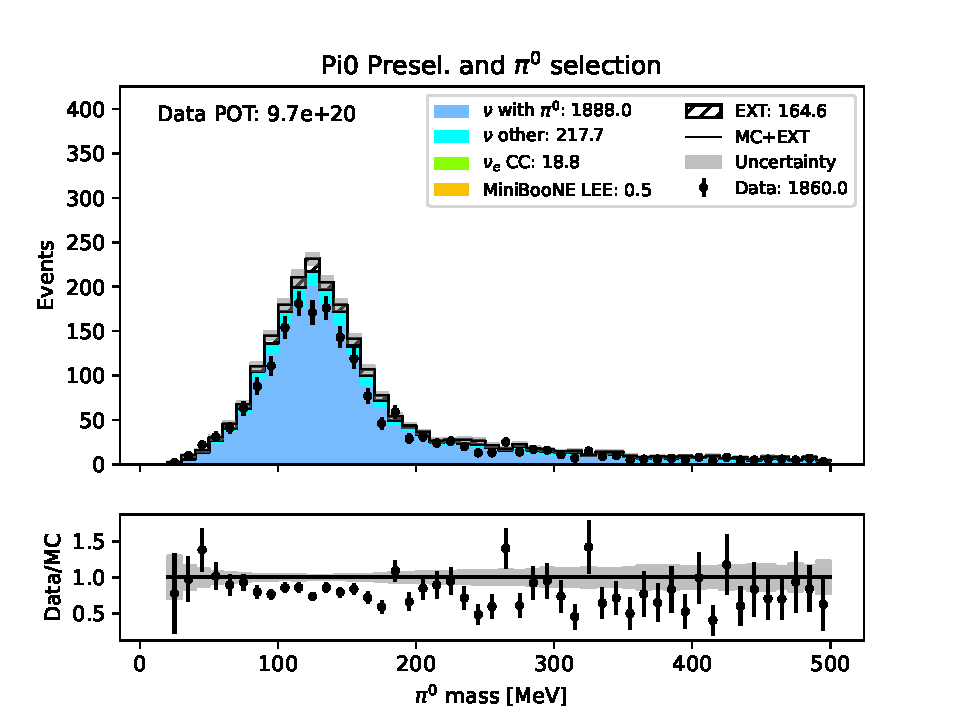
\includegraphics[width=\linewidth]{technote/Sidebands/Figures/TwoShowerSideband/two_shr_sideband_pi0_mass_Y_corr_run1234b4c4d_PI0_PI0.pdf}
        \caption{Reconstructed $\pi^0$ mass, runs 1-5.}
    \end{subfigure}%
    \begin{subfigure}{0.33\linewidth}
        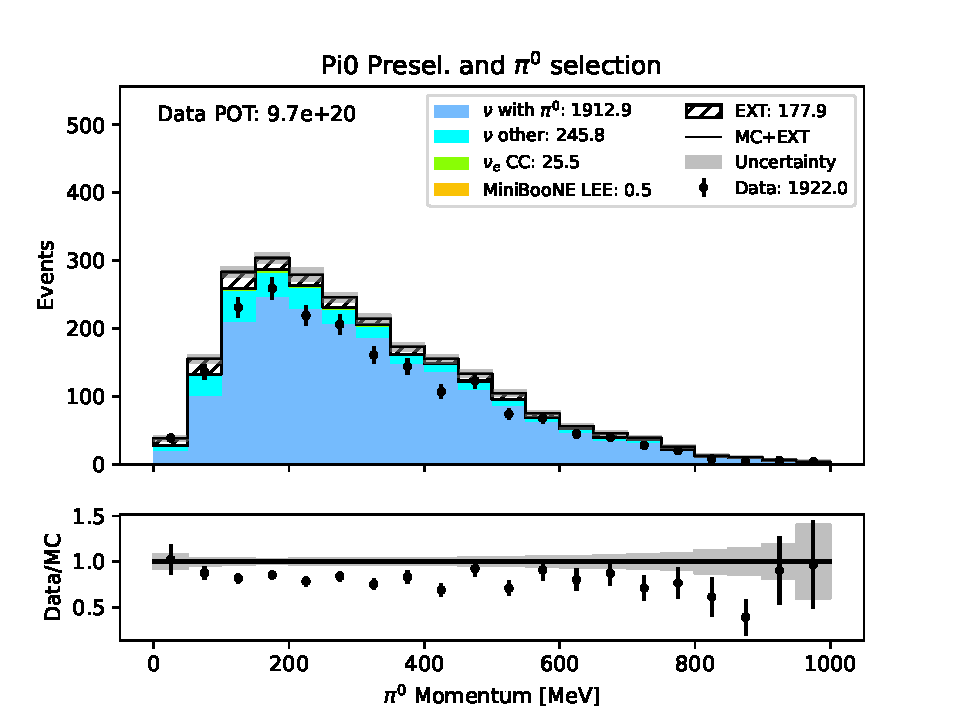
\includegraphics[width=\linewidth]{technote/Sidebands/Figures/TwoShowerSideband/two_shr_sideband_pi0momentum_run1234b4c4d_PI0_PI0.pdf}
        \caption{Reconstructed $\pi^0$ momentum, runs 1-5.}
    \end{subfigure}%
    \begin{subfigure}{0.33\linewidth}
        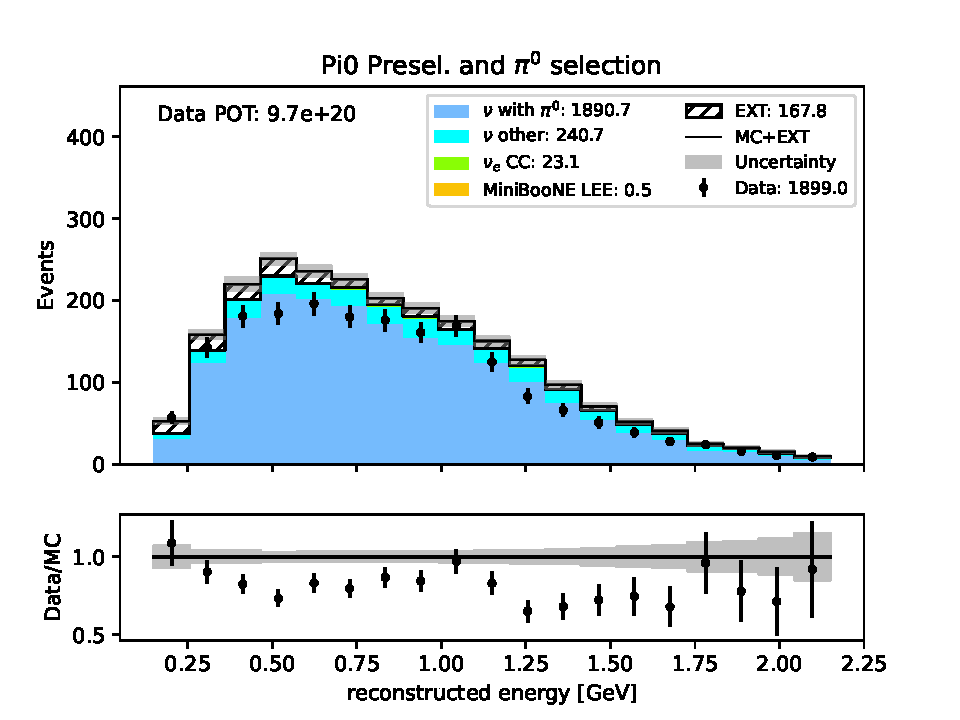
\includegraphics[width=\linewidth]{technote/Sidebands/Figures/TwoShowerSideband/two_shr_sideband_reco_e_run1234b4c4d_PI0_PI0.pdf}
        \caption{Reconstructed neutrino energy, runs 1-5.}
    \end{subfigure}
    \caption{Data and MC simulation comparisons after applying the full $\pi^0$ selection from Appendix~\ref{appendix:Pi0Selection} to data from the two shower sideband.}
    \label{fig:Pi0Sideband}
\end{figure}